\section{Zebrafish lines}
Calcium imaging experiments were carried out in zebrafish expressed \textit{Tg(HuC:H2B-GCaMP6s)} (Ahrens lab, Janelia farm). In this line, the \textit{HuC} promoter drives pan-neuronal expression of nuclear localised \textit{GCaMP6s} (these fish will be referred to as \textit{nls-GCaMP6s}). In addition,  \textit{nls-GCaMP6s} zebrafish that were null for genes encoding two isoforms of the NR2A subunit of the NMDAR (\textit{grin2aa -/-; grin2ab -/-}) were also imaged, this line will be referred to as the \textit{grin2a} \gls{dko}. To maximize optical clarity for imaging these fish were also compound \textit{roy;nacre} double homozygous mutants (\textit{casper}) larvae which lack melanocyte and iridophore pigmentation (\cite{White2008}). Behavioural experiments were performed using wild type (WT AB) fish generated by the mass embryo production service provided by the King's College London fish facility.

All larvae were raised at 28.5°C in Danieau solution (58mM NaCl, 0.7 mM KCl, 0.4 mM MgSO4, 0.6 mM Ca(NO3)2, 5 mM HEPES, pH 7.6) and were exposed to a 14 hour ON/10 hour OFF light/dark cycle. Larvae were fed daily from 5 \gls{dpf} using live rotifiers.  This work was approved by the local Animal Care and Use Committee (King’s College London), and was carried out in accordance with the Animals (Experimental Procedures) Act, 1986, under license from the United Kingdom Home Office.

\section{Generating the \textit{grin2a} double knock out in the \emph{nls-GCaMP6s} background}
\subsection{Breeding crosses}
Zebrafish posses two genetic paralogs encoding the NR2A subunit known as \textit{grin2aa} and \textit{grin2ab}. To create a DKO of the NR2A NMDAR subunit, both paralogs were targeted by \glspl{talen} that were designed to recognise start of exon 1, resulting in double strand breaks.  This caused a frame shift in both genes leading to a premature stop codon and a predicted truncated protein. This line was initially generated by Dr Paul Hunter in the \textit{HuC:GCaMP5} background, in which GCaMP is cytosolic. To compare functional imaging data in these mutants with fish expressing \emph{nls-GCaMP6s} this \gls{dko} needed be crossed with the \emph{nls-GCaMP6s} transgenic. To this end, \textit{grin2aa$_{(-/-)}$; grin2ab$_{(-/-)}$; HuC:GCaMP5$_{(-/+)}$} fish were out crossed with \gls{wt} fish containing no fluorescent reporter and their offspring screened for  non-fluorescence. The resulting \textit{grin2aa$_{(-/+)}$; grin2ab$_{(-/+)}$;  HuC:GCaMP5$_{(-/-)}$}  fish were incrossed and their offspring were genotyped by sequencing exon 1 to identify fish that were homozygous null for both \textit{grin2a} genes. These were then out crossed to the \emph{nls-GCaMP6s} line and their offspring incrossed. The resulting offspring were repeatedly incrossed until offspring expressed high levels of GCaMP fluorescence and were homozygous null for both \textit{grin2a} mutations  (\textit{grin2aa$_{(-/-)}$; grin2ab$_{(-/-)}$; nls-GCaMP6s $_{(+/+)}$}). 

\subsection{Genotyping}
For genotyping, adult suspected Grin2a mutants were temporarily anaesthetised in 0.025\% MS-222 (Sigma-Aldrich, catalog number: 886-86-2) in system water, and small tail samples were obtained. These samples were lysed in eppendorf tubes containing an alkaline buffer (25 mM NaOH; 0.2 EDTA) at 95$^{\circ}$C for 20 minutes. Each of the \textit{grin2a} genes were then amplified by \gls{pcr}. The PCR mix contained 12.5 $\mu$L platinum Hot start PCR 2x master mix, 0.5 $\mu$L forward primer (10 $\mu$M), 0.5 $\mu$L reverse primer (10  $\mu$M), 2 $\mu$L of genomic DNA and 9.5 $\mu$L nuclease free water. The PCR was run for 40 cycles with an annealing temperature of 58$^{\circ}$C. To ensure that DNA was amplified 5 $\mu$L of PCR product was run on a gel, and following the presence of a $\sim$450 bp band, was purified and sent for sequencing (Source Bioscience, Cambridge UK). For the PCR and sequencing the primers were as follows:



\begin{itemize}
    \item \textit{grin2aa}:
    \begin{itemize}
        \item  forward primer: 5'-GCAGCAAGGAGCATTCAG-3'
        \item  reverse primer: 5'-CTCTGTCAGAGATGTAGCGAG-3'
        \item  forward sequencing primer: 5'-GTATGCAGCAAGGAGCATT-3'
    \end{itemize}
    \item \textit{grin2ab}:
    \begin{itemize}
        \item   forward primer: 5'-GAACAGAGCGCAATCCC3-3'
        \item   reverse primer: 5'-CCAGTCCATGCAGTCTCTG-3'
        \item  forward sequencing primer: 5'-TGAATCGGTGCATGCCAAG-3'
    \end{itemize}
\end{itemize}
 
 Homozygous mutants were identified as having sequences identical to those in (\textbf{Figure \ref{fig:R2_F5}}) whereas heterozygous fish had double peaks in the sequencing data after the mutation site.

\section{Rearing protocol: Environmental enrichment by gravel rearing}
To assess the impact of visual experience on the development of naturalistic behaviour and visual system development, zebrafish were raised in different visual environments. Under laboratory conditions embryonic zebrafish usually develop in a petri dish placed on a shelf within an incubator. These rearing conditions lack many of the natural features of that zebrafish in the wild would usually experience (\cite{Engeszer2007ZebrafishField}). Therefore zebrafish were either raised under typical lab conditions (normally reared - \acrshort{nr}) or the petri dish rested on a bed of gravel (gravel reared - \acrshort{gr}). Gravel rearing the fish adds many of natural visual features that are lacking from the NR condition, creating an enriched environment. Gravel rearing started was started from 0-1 \gls{dpf}, before \glspl{rgc} begin to innervate the tectum at 2-3 \gls{dpf} (\cite{Burrill1994DevelopmentRerio}). Both conditions were fed rotifers (live prey) daily from the evening of 4 \gls{dpf} onwards.

\section{Functional imaging of spontaneous and visual evoked activity}
\subsection{Volumetric 2-photon calcium imaging}
To record neural activity in the tectum zebrafish of either sex were mounted in 2\% low melting point agarose in Danieau water with their dorsal side facing up on a custom built imaging slide and were submerged in Danieau water. These fish were left for 1 hour in the light so that the fish could settle, reducing drift while imaging. Neural activity was monitored by imaging the calcium dynamics of between 4000-6000  neurons in both tectal hemispheres with a custom built 2-photon microscope (Independent NeuroScience Services). Excitation was provided by a Mai Tai HP ultrafast Ti:Sapphire laser (Spectraphysics) tuned to 940nm. Laser power at the objective was kept below 15 mW for all fish. Emitted light was collected by a 16x, 1 NA water immersion objective (Nikon) and detected using a gallium arsenide phosphide detector (ThorLabs). Images (256 x 256 pixels) were acquired at a frame rate of 60Hz by scanning the laser in the x-axis with a resonant scanner and in the y-axis by a galvo-mirror. To enhance signal-to-noise every 2 frames for each focal plane were averaged. The focal plane was adjusted in 15$\mu$m steps using a piezo lens holder (Physik Instrumente). This allowed for volumetric data consisting of 5 focal planes to be collected at a volume rate of 4.8Hz. Scanning and image acquisition were controlled by Scanimage Software (Vidrio Technologies).

\subsection{Recording and analysis of spontaneous tectal activity}
To record spontaneous activity from the optic tectum mounted fish were placed in total darkness and volumetric calcium imaging was performed. To reduce transient neural activity that may be induced by the transition into this environment fish were allowed to adjust to the total darkness for $\sim$ 40 mins. To look at the development of spontaneous activity fish from 3, 5, 7 \gls{dpf} were imaged. All imaging experiments were conducted at 7 dpf.


\clearpage
\subsubsection{Preprocessing}
\newline
{\medium \textit{Image registration}\par}
Any recordings that showed drift in the z-plane were discarded. All other recordings where corrected for x and y drift by aligning every frame of the movie to the first image. This registration was performed using a nonrigid body alignment algorithm contained within the SPM8 plugin for MATLAB (\textcolor{blue}{http://www.fil.ion.ucl.ac.uk/spm/software/spm8}). Whilst this alignment corrected for slow drift of the fish caused by the agarose it could not correct for high velocity movements generated by the fish attempting to swim. This movement exceeds the
scanning rate of the microscope causing shearing of the image. As a result these frames were unusable and were manually removed.

\newline
{\medium \textit{Cell segmentation}\par}
Unlike cytosolyic GCaMP, the \emph{nls-GCaMP6s} line labels neurons in way that gives minimal overlap between neighbouring cells, reducing the likelihood of individual pixels containing mixed signals. Uniform expression within the nucleus results in an image that can be readily segmented, allowing for the detection of regions of interest corresponding to each neuron. Segmentation was performed on an average projection of the movie that had been smoothed with a 2D guassian kernel using a custom C++ script written by Giovanni Diana, Meyer Lab (\cite{Diana2019BayesianAssemblies}). Due to low pixel resolution within the images this segmentation algorithm takes into account both the morphology of the nucleus and the correlation of pixels within a segment, resulting in segmentation of cells that are active in nearly all cases. This produces a mask of labels that can be used to extract the time series for each neuron by averaging together all pixels with the same segmentation label for each frame of the movie. This has two distinct advantages over pixel wise analysis:
1) the traces for each neuron are less noisy than single pixels and 2) the number of
time series are reduced from 262144 x 5 pixels to  $\sim$ ~1500-3500 neurons, reducing the
computational load for subsequent analysis.

{\medium \textit{Detecting neuronal firing events from the fluorescence trace.}\par}
Raw fluorescence traces are built from a composite of signal from the calcium probe, low frequency fluctuations in baseline fluorescence (caused by bleaching of the calcium probe and z axial drift) and high frequency imaging noise.  Therefore, to quantify properties of neural responses the signal needed to be decomposed and the calcium signal extracted.
Furthermore, the decay of the GCaMP6s response is slow and is thought to be even slower when localized to the nucleus (\cite{Chen2013, Vladimirov2014}). This is likely to cause artefactual correlations. For example, two neurons firing a few seconds apart would appear to be correlated due to the slow kinetics of the probe. Therefore to examine temporal correlations, or the identify of neural assemblies (defined as synchronous groups of neurons), the time frames where neurons were most likely to be active needed to be inferred independently from the slow decay of the calcium probe.

For this purpose calcium signals were separated from baseline activity by using a a custom built R script, writtern by Giovanni Dianna, Meyer Lab (\cite{Diana2019BayesianAssemblies}). Briefly, this algorithm implements a \gls{hmm} to decompose the raw fluorescence into 1) the neuron activity state $S_{t}$ at time $t$ which is drawn from a Bernoulli process, 2) the background $B_{t}$ which is a Gaussian Markov process and 3) the imaging noise which is drawn from a Gaussian distribution.  Calcium signals are drawn from a normal distribution when the neuron activity state $S_{t}$ = 1 and follows an exponential decay when $S_{t}$ = 0. The values with maximum likelihood are then calculated conditional to the previous time points.  This processing gives both a calcium signal where noise and drifting baseline are absent and a binarised trace where a 1 represent a timepoint that the neuron was active and 0 when it is inactive. It is important to note that this binarised trace is not equivalent to actual spikes (action potentials), instead, it represents time points where there is maximum likelihood of the neuron being active. The calcium trace is subsequently used to calculate single neurons response properties such as response amplitude and duration whereas the binarised trace was used for correlations and identification of neural assemblies.

\subsubsection{Bayesian inference of neural assemblies}

Identification of spontaneously active neural assemblies in the optic tectum was achieved by using a Bayesian inference method called BINA (this method is explained in more detail in \textbf{Chapter 3} but for a full description see \cite{Diana2019BayesianAssemblies}). This method used a custom built C++ script, developed by Giovanni Dianna, Meyer Lab. In this method, a generative hierarchical model of synchronous activity is used to describe the organization of neurons into assemblies. Using Bayesian inference to infer the parameters of this model, this method provides a simultaneous estimation of assembly composition and within-assembly statistical features, such as the levels of activity, noise and assembly synchrony. 

The time taken to run this method is strongly influenced by the size of the activity matrix (neurons x frames) and the spontaneous activity recordings contained thousands of timepoints where few/no neurons firing. Therefore to speed computation times only frames with synchronous activity in more than 15 cells were used. For all recordings this threshold was used to select for synchronous activity events that had low probability (p < 0.02) of being random. This reduced compute times from over a week to 12-24hrs per dataset.

To approximate the probability distributions over the models parameters, BINA obtains samples using a Markov Chain Monte Carlo method known as a Gibbs sampler. This sampler randomly "walks" around the parameter space, preferentially sampling values which have higher probabilities. Since the Gibbs sampler initialises with random values, it takes a number of iterations before the sampler convergences on the posterior probability distribution. This convergence point could be identified looking by plotting log likelihood for each sample and observing a stable trace. Convergence was typically reached after 400,000 samples therefore each dataset was run for 600,000 samples, ensuring that convergence was definitely reached. The last 200 of these samples were then used as an approximation of the posterior probability distributions for each of the parameters. Neurons that could be assigned to an assembly in 99\% of these samples were treated as neurons that could be assigned to a single assembly. 

Metrics quantifying the structure and dynamics of the assemblies either utilised the model parameters directly or were calculated from them. All assembly metrics are explained throughout the results chapters. All statistical analysis of neural assemblies parameters across development and between genotypes were analysed in R. All statistical tests are reported throughout the chapters as they are used.

\subsubsection{Identifying correlated sub-networks of tectal assemblies}

To look at the organisation of correlated activity between tectal assemblies, pair-wise correlations were calculated between each assembly pair using the inferred time series of assembly activations that were inferred using the BINA method and this process was repeated for each sample of the posterior. A graph describing the assembly correlation was then constructed by adding a edge between all assembly pairs which has a positive correlation in over 95\% of the samples. This graph could then be clustered into subnetworks of correlated assemblies using the Girvan-Newman method (\cite{Newman2004FindingNetworks}) as implemented in the igraph R package (\cite{Csardi2006TheResearch}).


\subsection{The virtual reality hunting assay: visually evoked activity and behaviour}
\subsubsection{Imaging setup}
In order to simultaneously image visually evoked activity in the tectum and  tail movements 7 \gls{dpf} zebrafish were mounted in 2\% agarose within a custom built perspex cylindrical chamber. The fish was positioned so that its right eye faced a semi-circular screen covered in a grey diffusive filter and the chamber was filled with Danieau solution. This screen occupied 153$^{\circ}$ X 97$^{\circ}$ of visual space in terms of azimuth and elevation and was positioned 20 mm away from the fish. Visual stimuli could then be projected onto this screen using a P2JR pico-projector (AAXA Tech). To avoid interference of the projected image with the signal collected by the detector, a red long-pass filter (Zeiss LP590 filter) was placed in front of the projector. In order to image the fishes tail movement the imaging chamber was placed in the center of a 3D-printed semicircular ring of infrared LEDs. The infrared light hitting the fish body was refracted and reflected downwards, through the clear bottom of the chamber, onto a hot mirror which in turn reflected the light into Chameleon 3 FLIR camera imaging at 400Hz. This camera was fitted with a shortpass 900nm filter which allowed infrared light to pass through while blocking light from the laser. The camera, microscope and visual stimulation were synchronised via a transistor-transistor logic pulse that was sent from the microscope on the first frame of image acquisition. In this setup the visual evoked activity in the fish tectum could be imaged by volumetic calcium imaging (as above) while tail movements were monitored by the camera below for 1 hr. 

\subsubsection{Visual stimuli}
Visual stimuli were generated using a custom C$^{++}$ script written by Giovanni Dianna, Meyer lab.  5$^{\circ}$ black spots were presented at three different locations in visual azimuth separated by 10$^{\circ}$ intervals (-10$^{\circ}$, 0$^{\circ}$, +10$^{\circ}$). 0$^{\circ}$ was defined as the center of the screen, orthogonal to the zebrafish body axis. These spots moved with motion that resembled rotifer movement within a neighbourhood (5$^{\circ}$ radius) at a speed of 30 degrees/sec. These stimulus parameters were selected because they have been shown to induce hunting behaviours in head fixed larval zebrafish.

These dots were presented in two blocks which differed in the background they were projected over. In one block the background was a picture of gravel and the other it was simply a grey screen (\textbf{figure \ref{fig:m1}A}). Both backgrounds were presented in monochrome meaning that they did not differ in their color spectrum. In these blocks each spot was presented a total of 17 times per block in 5 second epochs, followed by 40 seconds of black screen. Importantly the movement of the dot was identical in each presentation Both the order of the blocks and order of these spots within the blocks were pseudo-randomised. Often fish can become startled by the initial stimulus. Therefore the fish were presented with a additional epoch, consisting of concentric rings moving inwards to a central point, prior to the experimental blocks. Furthermore, both the background and the dots faded in and out over the course of half a second to minimise any startle effects but that may be caused by sudden changes in the stimulus.

To understand what features of the background may be causing any changes in activity between these two blocks certain visual features were calculated to understand differences between the two backgrounds more fully. Firstly, contrast has been shown to be important for the detection of prey (\cite{Bianco2011}) with hunting behaviours being more likely to be initiated at greater contrasts therefore the mean difference in luminance between the background and the prey-like dots was calculated. This showed that the textured background had less contrast between the stimuli and background when compeared to the the grey background (\textbf{figure \ref{fig:m1}B}). However, the textured background has lots of local variance in luminance which could create high localised contrast between the stimulus and background. Therefore the difference between each pixel in the background and the stimulus was calculated. This showed that all pixel wise local contrast was less in the textured background, this should make it more difficult for the fish to detect the prey against the textured background. In addition, the power spectrum of difference spatial frequencies in the two backgrounds was calculated. The grey background, unsurprisingly had no different spatial frequencies. The textured background on the other had showed a wide range of different spatial frequencies, and resembled distributions that are typical of natural scenes (\cite{VanderSchaaf1996ModellingInformation}). Therefore it is possible that the differences in visually evoked activity between the two blocks may be driven by these differences in spatial frequencies between the two backgrounds as all other stimulus features are constant and differences in contrast are greater in the grey background.




\begin{figure}[!htb]
        \center{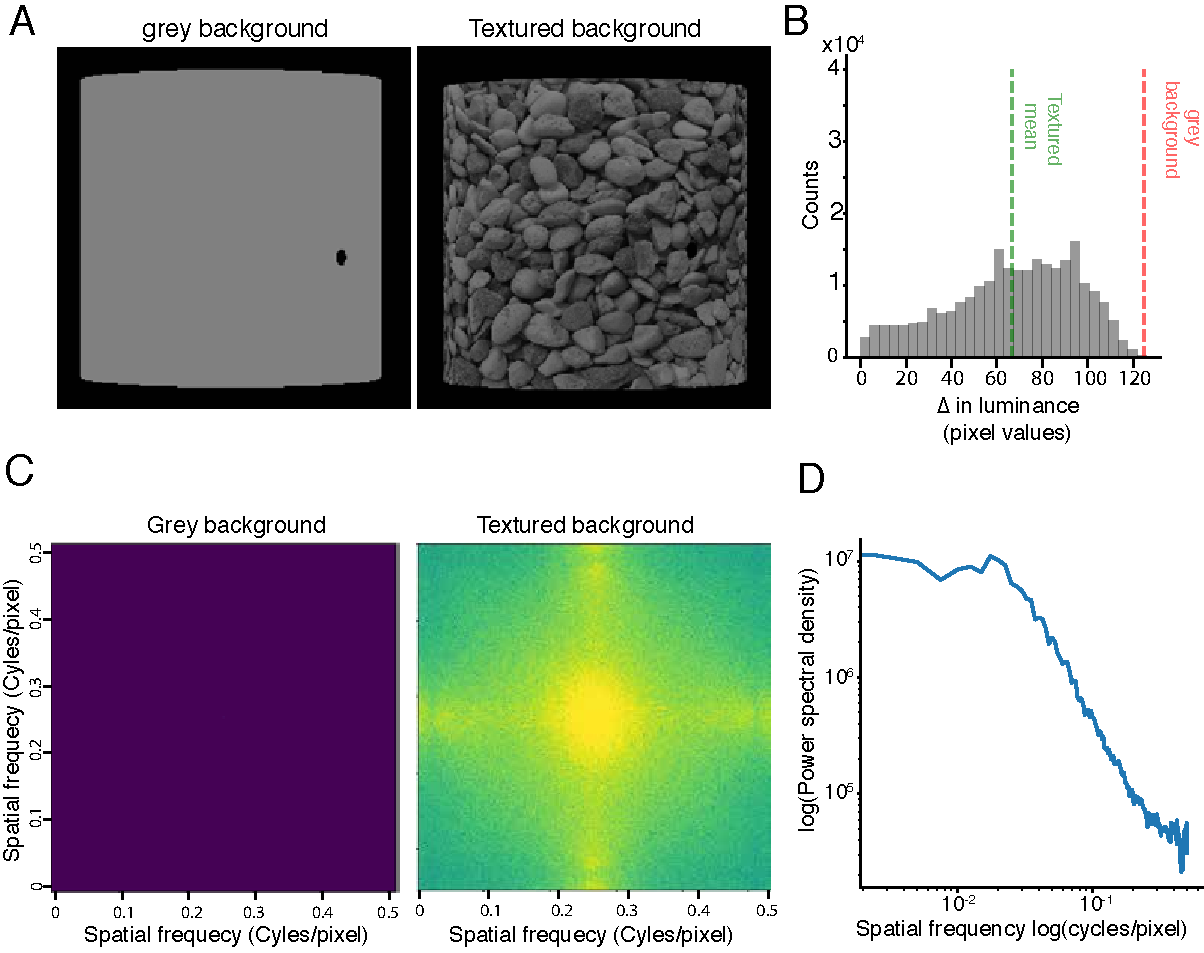
\includegraphics[width = 0.8\paperwidth]{Figures/m1.pdf}}
        \caption[\label{m1} \textbf{The difference in the statistics of the background between the two presented stimuli.}]{\label{fig:m1} \textbf{The difference in the statistics of the background between the two presented stimuli.  (A)} Two images showing a 5 deg spot being presented either over a grey background or a textured background. These stimuli were projected onto a curved screen positioned in front of the fishes eye \textbf{(B)} A histogram showing the change in luminance between the black dot and the background. The grey bins indicate the distribution of localised differences in luminance between the stimulus and pixels within the textured background. The green dotted line shows the the mean difference between the textured background and stimulus. The red line shows the difference in luminance between the grey background and the stimulus.  \textbf{(C)} Matrices showing the distribution of spatial frequencies in each background. \textbf{(D)} Power spectral density plot of the spatial frequencies shown in C. Only the textured background has been plotted as no spatial frequency changes were present in the grey background.}
      \end{figure}

\subsubsection{Preprocessing of visual evoked neural activity}
All data obtained from the virtual reality hunting assay was analysed using a custom written Python script. Visually evoked functional imaging data was both aligned and segemented using the Suite2p Python package (\textcolor{blue}{https://mouseland.github.io/suite2p}, \cite{Pachitariu2016Suite2p:Microscopy}).  The fluorescence level can vary between cells and change over the course of imaging due to bleaching and drift. Therefore the raw fluorescence for each cell, $F(t)$, was  normalised by calculating the $\Delta F/F(t)$ for each time $t$. This was defined as:

\begin{equation}
    \frac{\Delta F}{F} = \frac{(F(t) - F_{0}(t))}{F_{0}(t)}
\end{equation}

Where $F_{0}$ is the fluctuating baseline fluorescence that was estimated by calculating the bottom 8$^{th}$ percentile of groups of frames using a sliding window of 400 frames and was then smoothed with a Gaussian kernel.  This gave a smooth baseline that was fitted to timepoints that were unlikely to be calcium events. 

Many normalised traces were found to contain no calcium events over the time course of imaging. These inactive cells were removed using a "min-max" procedure. In this procedure a sliding window smaller than the typical duration of a calcium event (5 frames) was rolled through the $\Delta F/F$, calculating the minima for each window. The maxima of these minima were then calculated for each trace. This allowed for active traces to be identified because if the window encountered a calcium event the maxmin would be high, due to the sustained deviation from baseline, whereas inactive traces that fluctuated around baseline would have a low maxmin. As a result, a maxmin threshold of 0.1 $\Delta F/F$ was found to distinguish between active and inactive cells in all imaged fish (as determined by visual inspection of the traces). Of these only a subset of neurons were found to be responding to the stimulus.

Some neurons, likely to be related to ongoing activity or behaviour, may negatively impact decoding performance because their activity is sporadic, creating noise for the decoder (\cite{Kahn2015ANeurons}). In order to assess the impact of these cells on decoding performance we distinguished neurons that were responding to the stimulus by comparing the activity of neurons to that of random noise model for each neuron. To do this neuron traces were first binarised by setting timepoints exceeding 2 standard deviations of the mean for each trace to 1 and all other timepoints to  0. If $x_{i}$ represents the activity state of the neurons at each time $i$, $s_{i}$ denotes whether a stimulus is being shown ($s_{i}$ = 1 if stimulus is being presented or $s_{i}$ = 0 if stimulus is not being presented) and N represents the number of frames, then a \gls{ncc} can be calculated for each neuron by:

\begin{equation}
    NCC = \frac{1}{N} \sum_{t = 1}^{N}s_{i}x_{i}
\end{equation}

A neuron that reliably responds to every frame that there is a stimulus presentation would therefore have a NCC = 1, whereas one that is only  active at times when no stimulus is presented would have an NCC = -1. To identify neurons that were not firing in response to the stimulus (ie. firing randomly) the NCC value for each neuron was compeared to the average NCC for its own random noise model. To do this the expected value of the NCC ($\langle NCC \rangle$) for each neuron was calculated as if it was firing randomly with the same firing probability. A neuron was identified as visually responsive if its NCC value exceeded three standard deviations of the $\langle NCC \rangle$ of its own random noise model. This gives a threshold for being visually responsive for each neuron whilst taking into account its own firing probability. 
 
\subsubsection{Decoding}
In order to decode stimulus identity from neural activity the mean response for each neuron ($N$) to each stimulus presentation ($E$) was calculated to give a $N$ X $E$ stimulus response matrix. Here each column represents the population response over all neurons for a single stimulus presentation. A separate vector of length $E$ contained labels corresponding to the stimulus that had caused each population response.
These could be used to train the decoder to predict the stimulus identity from the population response. 

Decoding was performed using two separate linear decoders, \gls{lda} and \gls{logreg} (for more details see \textbf{Chapter 4}). Both decoders were trained using a leave-one-out cross validation strategy,  where a single population vector and it's corresponding label were removed from the training data set for testing. This leave-one-out procedure was repeated for all population vectors and the decoding performance was measured as the percentage of correctly decoded classes. All cross-validation and decoding steps were implemented in Python using the scikit learn library (\textcolor{blue}{https://scikit-learn.org/}).


\subsubsection{Tracking of tail movement and analysis}
The tail was tracked from behavioural recordings using \gls{dlc}, a \gls{cnn} designed for behavioural tracking (\cite{Mathis2018DeepLabCut:Learning}). This CNN uses a Resnet50 architecture that had been pretrained on tens of thousands of natural images (ImageNet database). Added downstream of this architecture are distinct readout (deconvolutional) layers which predict the probability that a labeled body part is in a particular pixel within the image. By initialising with pretrained weights DLC is able to transfer this learning to the tracking task, yielding highly accurate estimates of body position from small training datasets and with fast training times (\cite{Mathis2018DeepLabCut:Learning}; \cite{Mathis2020DeepNeuroscience}). 

In order to train this network, 250 frames from 3 different tail recordings of spontaneous tail movement were selected for labeling, these contained a variety of images of the tail at different phases of movement. For each of these frames eight positions along the tail were manually labeled, these positions were: the center of the fish's body (swim bladder), its tail tip and 6 evenly spaced locations between them. The \gls{cnn} was then trained on 200 frames of this labeled dataset for 250,000 iterations ($\sim$2 hours, Google Colab GPU). The remaining 50 labeled frames were used as a test set to assess the accuracy of the model. Test label prediction error was < 8 pixels, this was less than the width of the tail in the image ($\sim$13 pixels) and was therefore deemed acceptable. 

To calculate the tail angle at each timepoint of the movie the labeled points were skeletonised by treating the regions between the markers as separate vectors (or bones). The angle between each of these vectors relative to the x-axis was calculated. This was then subtracted from the average angle for each of these bones in the first 200 frames of the movie (prior to any movement of the tail). This gave the angle between the midline of the tail and each of the bones at each frame. The sum of these angles was then taken to give a trace that represented the total tail angle relative to the midline.

To automatically detect swim bouts, the first derivative of the total tail angle was calculated and was then smoothed with a Gaussian kernel of 20 frames. This had the effect of dilating neighbouring tail beats, creating a series of continuous positive values, which could then be binarised into segmented bouts using a threshold of 0.2 (arbitrary activity units). The peak of the first turn in each swim bout was used to calculate metrics of t. These quantified whether the turn fell within an epoch, its direction relative to the stimulus, it's latency relative to the epoch onset and tail angle.  


\section{Prey capture behavioural assay}
Hunting performance of zebrafish larvae was assessed using a hunting assay. For this assay rotifers were pipetted into 35mm petri dishes containing 3 ml of Danieau solution. These dishes were then placed within a custom built infrared LED ring (835nm) and and then imaged using a Chameleon 3 FLIR camera (30Hz) for 30 seconds. After this initial recording either GR or NR 7 \gls{dpf}  zebrafish larvae were added to the dish and were placed on either a gravel background or over a piece of white paper. The fish were then allowed to hunt over this background for 30 mins and then recorded again to assess how many rotifers the fish had consumed. Prior to recording both groups of fish were placed on the testing background for 40 mins to allow the fish to acclimatise to the novel visual background.

As some rotifers can be obscured by the side of the dish the 30 recordings were separated into 5 second segments and the mean count was taken. As the rotifers move around by swimming this ensured that rotifers who were at the side of the dish could be counted at other points in the movie. For these manual counts each frame in a segment was coloured in a different color and superimposed, this enabled rotifers to be distinguished from debris in the dish based on their swimming trajectory. All movies were assigned a random ID prior to counting using a custom built R script, blinding the counter to the experimental condition. Some group wise data from these experiments was non-normally distributed. Therefore group comparisons were analysed using pair wise Man-Whitney U-tests with Bonferroni corrections.